\section{On Predicting the Future}
\label{sec:predicting_future}

My goal in this article is to make accurate predictions of the future of
automatic speech recognition. Before I begin, I'd like to share some
findings on the general problem of predicting the future. These findings are
inpsired by one of the great forecasters, Richard Hamming. Hamming in \emph{The
Art of Doing Science and Engineering}~\citep{hamming1997art} makes many
predictions, many of which have come to pass. Here are a few examples:
\begin{enumerate}
    \item He stated that by ``the year 2020 it would be fairly universal
        practice for the expert in the field of application to do the actual
        program preparation rather than have experts in computers (and ignorant
        of the field of application) do the program preparation.''
    \item On neural networks he claimed that they ``represent a solution to
        \emph{the programming problem}'', and that ``they will probably play a
        large part in the future of computers''~\citep[chp. 4]{hamming1997art}.
    \item Haming was well ahead of the curve in computing. He advocated of
        general purpose rather than special purpose hardware, digital over
        analog, and high-level programming languages all long before the field
        had decided one way or another~\citep[chps. 2 and 4]{hamming1997art}.
    \item He anticipated the use of fiber-optic cables in place of copper wire
        for communication well before the switch actually took
        place~\citep[chp. 21]{hamming1997art}.
\end{enumerate}

These are just a few examples of Hamming's extraordinary prescience. Why was he
so good at predicting the future? Here are a few observations which I think were key to his ability:

{\bf Practice.} One doesn't get good at predicting the future without actually
practicing at it. Hamming practiced. He reserved Friday afternoon of every week
for ``great thoughts'' in which he mused on the future. But he didn't just
predict in isolation. He made his predictions public, which forced him to put
them in a communicable form and held him accountable. For example, in 1960
Hamming gave a talk titled ``The History of Computing to the Year 2000'' (you
may recognize the title).

{\bf Focus on fundamentals.} In some ways, forecasting the future is really
just understanding the present more than those around you. This requires not
just a depth in one field but non-trivial breadth. This also requires the
ability to rapidly assimilate new knowledge. Mastering the fundamentals builds
a strong foundation for both.

{\bf Open mind.} Probably the bmost important trait Hamming exhibited and, in
my opinion the most difficult to learn, was his ability to keep an open mind.
Keeping an open mind requires constant self-vigilance. Having an open mind one
day does not guarantee having it the next. Having an open mind with respect to
one scientific field does not guarantee having it with respect to another.
Hamming recognized for example that one may be more productive in an office
with the door closed but he kept his door open as he believed an ``open mind
leads to the open door, and the open door tends to lead to the open
mind''~\citep[chp. 30]{hamming1997art}.

I'll add to this a few of more thoughts. First, the rate of change of
technology is increasing. This makes it harder to predict farther into the
future today than it was 50 or 100 years ago. These days predicting the
evolution of a field even ten years out strikes me as a challenge. Hence that's
the time frame I'm choosing to work with.

A common saying about technology forecasting is that short-term predictions
tend to be overly optimistic and long-term predictions tend to be overly
pessimistic. This is often attributed to the fact that progress in technology
has been exponential. Figure~\ref{fig:exponential_growth} shows how this can
happen if we linearly extrapolate from the present with an overly optimistic
growth rate. The key drivers of progress in speech recognition over the
previous decade (2010-2020) underwent exponential growth. These include both
compute (e.g. floating-point operations per second) and dataset sizes. Whether
or not figure~\ref{fig:exponential_growth} applies to speech recognition for
the coming decade remains to be seen. We may continue to see rapid progressing
in compute and data, or we may be on a sigmoidal curve and approaching the
saturation point.
%% TODO tie this in with the rest of the work

I've attempted keep these in mind when assessing the
future of speech recognition for the rest of this decade.

\begin{figure}
    \centering
    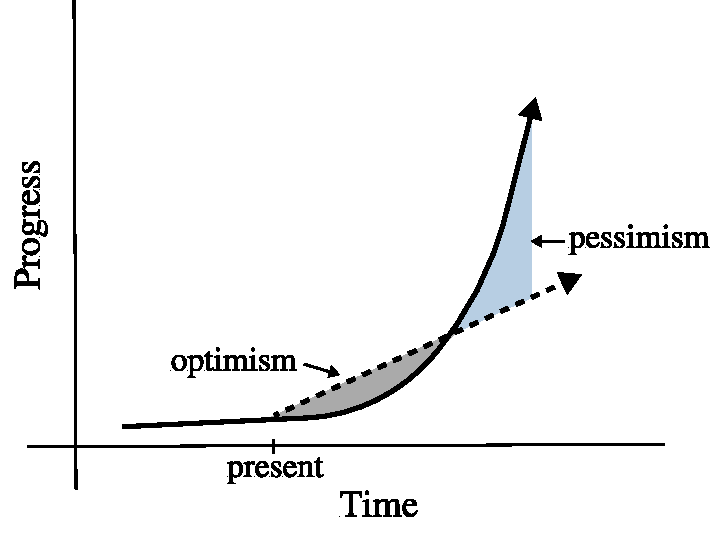
\includegraphics[width=\linewidth]{figures/exponential_growth}
    \caption{TODO}
    \label{fig:exponential_growth}
\end{figure}

Second, as a hedge, I want to be clear that I think predicting the future is
\emph{hard}, and I am no expert at it. I'm sure a lot of the following
predictions prove wrong. In some ways the more controvesail predictions I make
are really more of an optimistic wishlist for the future. On that note, let me
close this section with the famous words of Alan Kay:
\begin{quote}
    \emph{The best way to predict the future is to invent it.}
\end{quote}
